

The STL uses iterators to navigate the elements of its container classes. Most containers include begin() and end() iterators. These are usually implemented as member functions that return an iterator object. The begin() iterator points to the initial container element, and the end() iterator points past the final element:

\hspace*{\fill} \\ %插入空行
\begin{center}
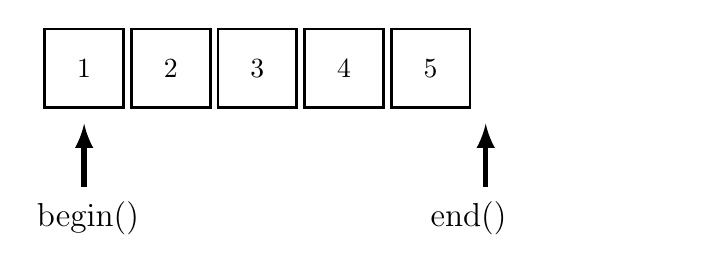
\begin{tikzpicture}
\foreach \x in {1,...,5} {
	\draw[line width=1pt] (1.1*\x,1) rectangle (1.1*\x+1,0) node[pos=.5] {\x};
}

\draw[line width=2pt][-latex] (1.6,-1.0) -- (1.6,-0.2);
\draw[line width=2pt][-latex] (6.7,-1.0) -- (6.7,-0.2);

\node[text width=3cm, font=\large] at (2.5,-1.4) {begin()};
\node[text width=3cm, font=\large] at (7.5,-1.4) {end()};
\end{tikzpicture}

Figure 4.1 – The begin() and end() iterators
\end{center}

The end() iterator may function as a sentinel for containers of indeterminate length.
We'll see some examples of that in this chapter.

Most STL containers define their own specific iterator type. For example, for a vector of int:

\begin{lstlisting}[style=styleCXX]
std::vector<int> v;
\end{lstlisting}

The iterator type would be defined as:

\begin{lstlisting}[style=styleCXX]
std::vector<int>::iterator v_it;
\end{lstlisting}

You can see how this could easily get out of hand. If we had a vector of vector of string:

\begin{lstlisting}[style=styleCXX]
std::vector<std::vector<int, std::string>> v;
\end{lstlisting}

Its iterator type would be:

\begin{lstlisting}[style=styleCXX]
std::vector<std::vector<int, std::string>>::iterator v_it;
\end{lstlisting}

Fortunately, C++11 gave us automatic type deduction and the auto type. By using auto, we rarely need to use the full iterator type definition. For example, if we need an iterator in a for loop, we can use the auto type:

\begin{lstlisting}[style=styleCXX]
for(auto v_it = v.begin(); v_it != v.end(); ++v_it) {
	cout << *v_it << '\n';
}
\end{lstlisting}

Notice the use of the dereference operator * to access the elements from the iterator. This is the same syntax you would use to dereference a pointer:

\begin{lstlisting}[style=styleCXX]
const int a[]{ 1, 2, 3, 4, 5 };
size_t count{ sizeof(a) / sizeof(int) };
for(const int* p = a; count > 0; ++p, --count) {
	cout << *p << '\n';
}
\end{lstlisting}

This also means that you can use a range-based for loop with either a primitive array:

\begin{lstlisting}[style=styleCXX]
const int a[]{ 1, 2, 3, 4, 5 };
for(auto e : a) {
	cout << e << '\n';
}
\end{lstlisting}

Or with an STL container:

\begin{lstlisting}[style=styleCXX]
std::vector<int> v{ 1, 2, 3, 4, 5 };
for(auto e : v) {
	cout << e << '\n';
}
\end{lstlisting}

The range-based for loop is just a shorthand for a for loop with iterators:

\begin{lstlisting}[style=styleCXX]
{
	auto begin_it{ std::begin(container) };
	auto end_it{ std::end(container) };
	for ( ; begin_it != end_it; ++begin_it) {
		auto e{ *begin_it };
		cout << e << '\n';
	}
}
\end{lstlisting}

Because iterators use the same syntax as a primitive pointer, the range-based for loop works the same with either container.

Notice that the range-based for loop calls std::begin() and std::end(), instead of directly calling the begin() and end() member functions. The std:: functions call the member functions to get the iterators. So, why not just call the member functions? The std:: non-member functions are designed to also work with primitive arrays. That's why a for loop works with an array:

\begin{lstlisting}[style=styleCXX]
const int arr[]{ 1, 2, 3, 4, 5 };
for(auto e : arr) {
	cout << format("{} ", e);
}
\end{lstlisting}

Output:

\begin{tcblisting}{commandshell={}}
1 2 3 4 5
\end{tcblisting}

For most purposes, I tend to favor the member function begin() and end() because they are more explicit. Others favor the std:: non-member functions because they are more general. Six or half-dozen; I suggest you pick a style and stick with it.

\subsubsection{Iterator categories}

Prior to C++20, iterators were divided into categories based on their capabilities:

% Please add the following required packages to your document preamble:
% \usepackage{multirow}
\begin{table}[H]
\centering
\begin{tabular}{|llllll|}
\hline
\multicolumn{5}{|c|}{\textbf{Iteratgor Category}} &
\multicolumn{1}{c|}{\textbf{Iterator Capability}} \\ \hline
\multicolumn{1}{|l|}{\multirow{5}{*}{\begin{tabular}[c]{@{}l@{}}Contiguous\\ Iterator\end{tabular}}} &
\multicolumn{1}{l|}{\multirow{4}{*}{\begin{tabular}[c]{@{}l@{}}Random\\ Access Iterator\end{tabular}}} &
\multicolumn{1}{l|}{\multirow{3}{*}{\begin{tabular}[c]{@{}l@{}}Bidirectional\\ Iterator\end{tabular}}} &
\multicolumn{1}{l|}{\multirow{2}{*}{\begin{tabular}[c]{@{}l@{}}Forward\\ Iterator\end{tabular}}} &
\multicolumn{1}{l|}{Input Iterator} &
\begin{tabular}[c]{@{}l@{}}·Read\\ ·Increment once\end{tabular} \\ \cline{5-6} 
\multicolumn{1}{|l|}{} &
\multicolumn{1}{l|}{} &
\multicolumn{1}{l|}{} &
\multicolumn{1}{l|}{} &
\multicolumn{1}{l|}{} &
\begin{tabular}[c]{@{}l@{}}·Increment multiple\\ times\end{tabular} \\ \cline{4-6} 
\multicolumn{1}{|l|}{} &
\multicolumn{1}{l|}{} &
\multicolumn{1}{l|}{} &
\multicolumn{2}{l|}{} &
·Decrement \\ \cline{3-6} 
\multicolumn{1}{|l|}{} &
\multicolumn{1}{l|}{} &
\multicolumn{3}{l|}{} &
·Random access \\ \cline{2-6} 
\multicolumn{1}{|l|}{} &
\multicolumn{4}{l|}{} &
\begin{tabular}[c]{@{}l@{}}·Contiguous storage\\ (such as an array)\end{tabular} \\ \hline
\multicolumn{6}{|l|}{When any of the above iterators can also write, they are called mutable iterators.} \\ \hline
\multicolumn{5}{|l|}{Ouput Iterator} &
\begin{tabular}[c]{@{}l@{}}·Write\\ ·Increment once\end{tabular} \\ \hline
\end{tabular}
\end{table}

These categories are hierarchical, where the more capable iterators inherit the capabilities of the less capable iterators. In other words, the input iterator can read and increment once. The forward iterator has the capabilities of the Input Iterator plus it can increment multiple times. The bidirectional iterator has those capabilities plus it can decrement. And on down the list.

The output iterator can write and increment once. If any of the other iterators can also write, it is considered a mutable iterator.

\subsubsection{Iterator concepts}

Concepts and constraints are new with C++20. A concept is simply a named constraint that restricts the types of arguments to a template function or class, and helps the compiler choose appropriate specializations.

Beginning with C++20, the STL defines iterators in terms of concepts instead of categories. Each of these concepts are in the std:: namespace.

\begin{table}[H]
\centering
\begin{tabular}{|l|l|}
\hline
\textbf{Concept} &
\textbf{Description} \\ \hline
indirectly\_readable &
\begin{tabular}[c]{@{}l@{}}An iterator can be read by the dereference\\ operator,*. This includes pointers, smart pointers,\\ and input iterators.\end{tabular} \\ \hline
indirectly\_writeable &
The object reference of the iterator is writable. \\ \hline
weakly\_incrementable &
\begin{tabular}[c]{@{}l@{}}This can be incremented with ++, but does not\\ preserve equality. For example, where a==b, ++a\\ may not equal ++b.\end{tabular} \\ \hline
incrementable &
\begin{tabular}[c]{@{}l@{}}This can be incremented with ++ and equality is \\ preserved.\end{tabular} \\ \hline
\begin{tabular}[c]{@{}l@{}}input\_or\_output\_\\ iterator\end{tabular} &
\begin{tabular}[c]{@{}l@{}}An iterator can be incremented and dereferenced.\\ Every iterator must satisfy this concept.\end{tabular} \\ \hline
sentinel\_for &
\begin{tabular}[c]{@{}l@{}}A sentinel iterator is used to find the end of an\\ object of indeterminate size, such as an input \\ stream.\end{tabular} \\ \hline
sized\_sentinel\_for &
\begin{tabular}[c]{@{}l@{}}A sentinel iterator may be used with another\\ iterator and the - operator to determine its\\ distance in constant time.\end{tabular} \\ \hline
input\_iterator &
An iterator that may be read and incremented. \\ \hline
output\_iterator &
An iterator that may be written to and incremented. \\ \hline
forward\_iterator &
\begin{tabular}[c]{@{}l@{}}This modifies input\_iterator to include\\ incrementable.\end{tabular} \\ \hline
\begin{tabular}[c]{@{}l@{}}bidirectional\_\\ iterator\end{tabular} &
\begin{tabular}[c]{@{}l@{}}This modifies forward\_iterator by adding\\ the ability by decrement with the -- operator, It\\ preserves equality.\end{tabular} \\ \hline
\begin{tabular}[c]{@{}l@{}}random\_access\_\\ iterator\end{tabular} &
\begin{tabular}[c]{@{}l@{}}This modifies bidirectional\_iterator by adding\\ support for the +,+=,-,-=, and {[}{]} operators.\end{tabular} \\ \hline
contiguous\_iterator &
\begin{tabular}[c]{@{}l@{}}This modifies random\_access\_iterator to indicate\\ contiguous storage.\end{tabular} \\ \hline
\end{tabular}
\end{table}

You can use these concepts to constrain the arguments of a template:

\begin{lstlisting}[style=styleCXX]
template<typename T>
requires std::random_access_iterator<typename T::iterator>
void printc(const T & c) {
	for(auto e : c) {
		cout << format("{} ", e);
	}
	cout << '\n';
	cout << format("element 0: {}\n", c[0]);
}
\end{lstlisting}

This function requires a random\_access\_iterator. If I call it with a list, which is not a random-access container, the compiler will give me an error:

\begin{lstlisting}[style=styleCXX]
int main()
{
	list<int> c{ 1, 2, 3, 4, 5 };
	printc(c);
}
\end{lstlisting}

The list iterator type does not support the random\_access\_iterator concept. So, the compiler gives me an error:

\begin{tcblisting}{commandshell={}}
error: no matching function for call to 'printc(std::__
cxx11::list<int>&)'
  27 | printc(c);
       | ~~~~~~^~~
note: candidate: 'template<class T> requires random_access_
iterator<typename T::iterator> void printc(const T&)'
  16 | void printc(const T & c) {
      |         ^~~~~~
note: template argument deduction/substitution failed:
note: constraints not satisfied
\end{tcblisting}

This is the error output from GCC. Your errors may look different.

If I call it with a vector, which is a random-access container:

\begin{lstlisting}[style=styleCXX]
int main()
{
	vector<int> c{ 1, 2, 3, 4, 5 };
	printc(c);
}
\end{lstlisting}

Now it compiles and runs without error:

\begin{tcblisting}{commandshell={}}
$ ./working
1 2 3 4 5
element 0: 1
\end{tcblisting}

While there are different types of iterators for different types of capabilities (and concepts), the complexity is there to support of ease of use.

With this introduction to iterators, let's now proceed with the following recipes in this chapter:

我们将讨论以下主题:

\begin{itemize}
\item 
Create an iterable range

\item 
Make your iterators compatible with STL iterator traits

\item 
Use iterator adapters to fill STL containers

\item 
Create a generator as iterators

\item 
Use reverse iterator adapters to iterate backward

\item 
Iterate objects of unknown length with a sentinel

\item 
Build a zip iterator adapter

\item 
Create a random-access iterator
\end{itemize}


